
% \begin{multicols}{2}

\begin{wrapfigure}{r}{0.5\linewidth-0.5\columnsep}
  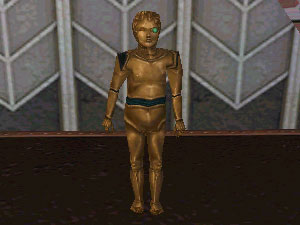
\includegraphics[width=\linewidth]{pip}
\end{wrapfigure}

\section{Forgotten Ghost Boy}

\minipage{0.5\linewidth-0.5\columnsep}
\flavorquote
{I can do it!}{Pip, last words}
\endminipage

\noindent{Pip is your property. You can use him as \textit{unseen servant} at will, though you can see him clearly and no one else can.}

You can also 1/day summon him as a \textit{ghost} for up to an hour, and he is invisible unless you wish him not to be. He can \textit{possess} people in or out of combat, but you will control the possessed person. If he “dies” in combat you must sacrifice blood to revive him.

% \newenvironment{PipFigure}
%   {\par\medskip\noindent\minipage{\linewidth}}
%   {\endminipage\par\medskip}

% \begin{PipFigure}
%   \centering
%   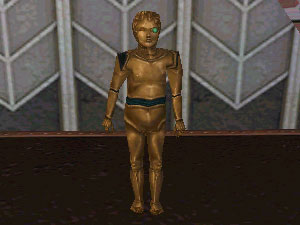
\includegraphics[scale=0.8]{pip}
% \end{PipFigure}

% \end{multicols}

\begin{figure}[b!]
% You can optionally not include the background by saying
% begin{monsterboxnobg}
\begin{monsterbox}{Pip’s Ghost}
  \begin{multicols}{2}
	\textit{Small undead, neutral evil}\\
	\hline
	\basics[%
	armorclass = 11,
	hitpoints  = 45,
	speed      = {0 ft., fly 40 ft.}
	]
	\hline
	\stats[
	STR = \stat{7}, % This stat command will autocomplete the modifier for you
	DEX = \stat{13},
	CON = \stat{10},
	INT = \stat{10},
	WIS = \stat{12},
	CHA = \stat{17}
	]
	\hline
	\details[%
	% If you want to use commas in these sections, enclose the
	% description in braces.
	% I’m so sorry.
	senses = {darkvision 60 ft., passive Perception 11},
	languages = {any languages Gumdrop knows},
	damageresistances = {acid, fire, lightning, thunder; bludgeoning, piercing, and slashing from nonmagical weapons},
	damageimmunities = {cold, necrotic, poison},
	conditionimmunities = {charmed, exhaustion, frightened, grappled, paralyzed, petrified, poisoned, prone, restrained}
	]
	\begin{monsteraction}[Ethereal Sight]
    The ghost can see 60 ft. into the Ethereal Plane when it is on The Material Plane, and vice versa.
  \end{monsteraction}
  \begin{monsteraction}[Incorporeal Movement]
    The ghost can move through other creatures and Objects as if they were difficult terrain. It takes 5 (1d10) force damage if it ends its turn inside an object.
	\end{monsteraction}
  \monstersection{Actions}
  \begin{monsteraction}[Withering Touch]
    \textit{Melee Weapon Attack:} +5 to hit, reach 5 ft., one target. \textit{Hit:} 17 (4d6 + 3) necrotic damage.
  \end{monsteraction}
  \begin{monsteraction}[Etherealness]
    The ghost enters the Ethereal Plane from The Material Plane, or vice versa. It is visible on The Material Plane while it is in the Border Ethereal, and vice versa, yet it can't affect or be affected by anything on the other plane.
  \end{monsteraction}
  \begin{monsteraction}[Possession (Recharge 6)]
    One humanoid that the ghost can see within 5 ft. of it must succeed on a DC 13 Charisma saving throw or be possessed by the ghost; the ghost then disappears, and the target is Incapacitated and loses control of its body. The ghost now controls the body but doesn't deprive the target of awareness. The ghost can't be targeted by any Attack, spell, or other effect, except ones that turn Undead, and it retains its alignment, Intelligence, Wisdom, Charisma, and immunity to being Charmed and Frightened. It otherwise uses the possessed target's Statistics, but doesn't gain access to the target's knowledge, Class Features, or proficiencies.
    \par The possession lasts until the body drops to 0 hit points, the ghost ends it as a Bonus Action, or the ghost is turned or forced out by an effect like the \textit{Dispel Evil and Good} spell. When the possession ends, the ghost reappears in an unoccupied space within 5 ft. of the body. The target is immune to this ghost's Possession for 24 hours after succeeding on the saving throw or after the possession ends.
  \end{monsteraction}
  \end{multicols}
\end{monsterbox}


% \subtitlesection{Slaadpole}
\end{figure}

% \begin{multicols}{2}
\twocolumn

\section{Slaad Dragon Hybrid}

\begin{quotebox}
	{She removes the cloth to reveal the little green slaad, or what was the green slaad. Still a small tadpole, it looks as though it’s been changed fundamentally. It’s hands and feet end in black scales and claws, the same shape a before but as though they have been made from different hide. Most striking, the color of the slaads eyes now mirror your own. Your true eyes, in shape and color. And for the first time you can understand the slaad’s cries not only telepathically, but vocally as well.}{}
\end{quotebox}
